\section{Tasks Status} % Seções são adicionadas para organizar sua apresentação em blocos discretos, todas as seções e subseções são automaticamente exibidas no índice como uma visão geral da apresentação, mas NÃO são exibidas como slides separados.

%----------------------------------------------------------------------------------------


\begin{frame}
  \frametitle{Conference Materials Status}

  \centering
  \renewcommand{\arraystretch}{1.15}

  \begin{table}
    \begin{tabular}{|p{0.38\textwidth}|c|p{0.42\textwidth}|}
      \hline
      \textbf{Task} & \textbf{Status} &  \\
      \hline

      \hspace{1.2em}\textbf{2026-10 Conference}
      & \pending & \href{https://www.overleaf.com/read/ngrqfgxjtxsh\#752747}{Simpósio IFUSP Presentation} \\
      \hline

      \hspace{1.2em}\textbf{2026-10 Conference}
      & \pending & \href{https://www.overleaf.com/read/bmsvqftfmrmh\#72805a}{AGORÁ Presentation} \\
      \hline

      \hspace{1.2em}\textbf{2026-11 Poster}
      & \pending & \href{https://www.overleaf.com/read/prxpvcsqhfdt\#7c9a4f}{3rd Schooll QC Poster} \\
      \hline

      \hspace{1.2em}\textbf{2026-12 Conference}
      & \pending & \href{https://www.overleaf.com/read/wvdxvvqstzcg\#e87182}{LASNPA Presentation} \\
      \hline

      \hspace{1.2em}\textbf{2026-12 Paper}
      & \pending & \href{https://www.overleaf.com/read/kxmvkdmchctm\#c1dd9c}{LASNPA Proceedings} \\
      \hline

      \hspace{1.2em}\textbf{2027-03 Conference}
      & \pending & \href{https://www.overleaf.com/read/zjpxtshjcqvr\#9ea901}{Quark Matter Presentation} \\
      \hline

    \end{tabular}
  \end{table}


  % \begin{table}
  %   \begin{tabular}{|p{0.58\textwidth}|c|p{0.22\textwidth}|}
  %     \hline
  %     \textbf{Task} & \textbf{Status} &  \\
  %     \hline

  %     \hspace{1.2em}\textbf{Journal Club - Automations}
  %     & \inprogressqqqq & \\
  %     \hline

  %   \end{tabular}
  % \end{table}
\end{frame}

\begin{frame}{Study Phases -- Dependencies}
  \centering
  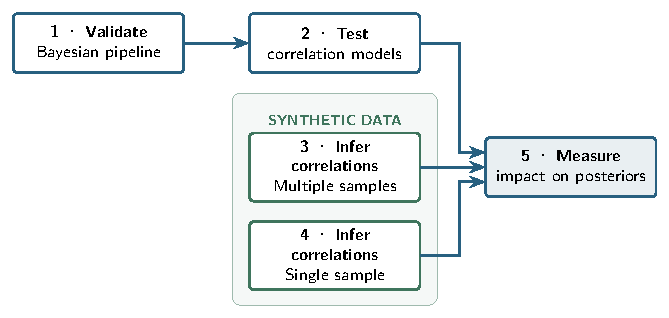
\includegraphics[width=0.96\textwidth,height=0.78\textheight,keepaspectratio]{diagrams/phase_dependencies.pdf}
\end{frame}

\begin{frame}[t]
\frametitle{Phase 1 -- Bayesian Pipeline Validation}

\centering
\renewcommand{\arraystretch}{1.12}
\small

\begin{tabular}{|p{0.58\textwidth}|c|p{0.16\textwidth}|}
\hline
\textbf{Task} & \textbf{Status} & \textbf{Output} \\
\hline

\hspace{1em}$\hookrightarrow$ Reproduce Mankolli et al. results
with the original JETSCAPE emulator
& \done & Reference \\
\hline

\hspace{1em}$\hookrightarrow$ Reproduce the same results with
the \texttt{hic\_bayes} emulator
& \pending & Validation \\
\hline

\hspace{1em}$\hookrightarrow$ Emulator closure test
& \pending & Validation \\
\hline

\hspace{1em}$\hookrightarrow$ MCMC convergence test
& \pending & Diagnostics \\
\hline

\hspace{1em}$\hookrightarrow$ Verify that model parameters are constrained
& \pending & Posteriors \\
\hline

\end{tabular}
\end{frame}

\begin{frame}[t]
\frametitle{Phase 2 -- Correlation Model Sensitivity}

\centering
\renewcommand{\arraystretch}{1.12}
\small

\begin{tabular}{|p{0.58\textwidth}|c|p{0.16\textwidth}|}
\hline
\textbf{Task} & \textbf{Status} & \textbf{Output} \\
\hline

\hspace{1em}$\hookrightarrow$ Au--Au-200 + d--Au-200:
Diagonal vs. CS vs. RBF correlation models
& \inprogressqqqqqq & Posteriors \\
\hline

\hspace{1em}$\hookrightarrow$ Compare posterior shifts,
credible intervals, and parameter correlations
& \inprogressqqqqq & Analysis \\
\hline

\hspace{1em}$\hookrightarrow$ \textbf{Question to answer:} What is the
appropriate correlation-length unit for an RBF covariance
spanning heterogeneous observables/bins?
& \pending & Study \\
\hline

\hspace{1em}$\hookrightarrow$ Quantify and compare the emulator-error
and experimental-error covariance matrices in the likelihood
& \pending & Analysis \\
\hline

\end{tabular}
\end{frame}

\begin{frame}[t]
\frametitle{Phase 3 -- Correlation Inference from Multiple Samples}

\centering
\renewcommand{\arraystretch}{1.12}
\small

\begin{tabular}{|p{0.58\textwidth}|c|p{0.16\textwidth}|}
\hline
\textbf{Task} & \textbf{Status} & \textbf{Output} \\
\hline

\hspace{1em}$\hookrightarrow$ Generate controlled synthetic
datasets with known covariance ($N$ samples; goal: $N=10$)
& \inprogressqqq & Dataset \\
\hline

\hspace{1em}$\hookrightarrow$ Classical correlation inference
& \pending & Benchmark \\
\hline

\hspace{1em}$\hookrightarrow$ Quantum-learning correlation inference
& \pending & Benchmark \\
\hline

\hspace{1em}$\hookrightarrow$ Classical vs. quantum comparison
against the known covariance
& \pending & Comparison \\
\hline

\end{tabular}
\end{frame}

\begin{frame}[t]
\frametitle{Phase 4 -- Single-Sample Correlation Inference}

\centering
\renewcommand{\arraystretch}{1.12}
\small

\begin{tabular}{|p{0.58\textwidth}|c|p{0.16\textwidth}|}
\hline
\textbf{Task} & \textbf{Status} & \textbf{Output} \\
\hline

\hspace{1em}$\hookrightarrow$ Study correlation approximations
when only one experimental sample is available
& \inprogressqqq & Heuristics \\
\hline

\hspace{1em}$\hookrightarrow$ Use reported uncertainty components
to constrain plausible correlation structures
& \pending & Models \\
\hline

\end{tabular}
\end{frame}

\begin{frame}[t]
\frametitle{Phase 5 -- End-to-End Bayesian Impact}

\centering
\renewcommand{\arraystretch}{1.12}
\small

\begin{tabular}{|p{0.58\textwidth}|c|p{0.16\textwidth}|}
\hline
\textbf{Task} & \textbf{Status} & \textbf{Output} \\
\hline

\hspace{1em}$\hookrightarrow$ Propagate inferred covariance
matrices through the Bayesian likelihood
\begin{itemize}
  \setlength{\itemsep}{0pt}
  \setlength{\parskip}{0pt}
  \item \textbf{Single sample:} CS, RBF, Zero, GP
  \item \textbf{Multiple samples:} Classical, Quantum
\end{itemize}
& \pending & Posteriors \\
\hline

\hspace{1em}$\hookrightarrow$ Quantify covariance-estimation error
$\rightarrow$ posterior error
& \pending & Final study \\
\hline

\end{tabular}
\end{frame}






% \begin{frame}
%   \frametitle{Correlated Uncertainty Study Tasks Status}

%   % Ajustes úteis em tabelas no Beamer
%   \centering
%   \renewcommand{\arraystretch}{1.15} % mais espaço vertical entre linhas

%   \begin{table}

% \begin{tabular}{|p{0.50\textwidth}|c|p{0.20\textwidth}|}
% \hline
% \textbf{Task} & \textbf{Status} & \textbf{Link} \\
% \hline
% \hspace{1.2em}\textbf{Correlation Inference Study - Classical Approach}
% & \inprogressqqq &  \\
% \hline
% \hspace{1.2em}\textbf{Correlation Inference Study - Quantum Learning Approach}
% & \pending &  \\
% \hline
% \textbf{Alice ins1222333 Studies} & & \\
% \hline
% \hspace{1.2em}\small$\hookrightarrow$ Uncertainty correlation effect & \done & \href{https://github.com/IFUSP-Heavy-Ions/hic-bayes/releases/tag/AtlasPbPb2760_mcmc_params-v0.1}{Plots} \\
% \hline
% \textbf{RHIC Au-Au/d-Au Studies JETSCAPE} & & \\
% \hline
% \hspace{1.2em}\small$\hookrightarrow$ Uncertainty correlation effect & \done & \href{https://github.com/IFUSP-Heavy-Ions/hic-bayes/releases/tag/AllDetectorsAuAu200_uncertainty_correlation-v0.1}{Plots}\\
% \hline
% \textbf{Atlas ins1759506 studies} & & \\
% \hline
% \hspace{1.2em}\small$\hookrightarrow$ Uncertainty correlation inference & \inprogressqqqq & \href{https://high-energy-physics-research.github.io/Gaussian-Process-Research/studies.html?nb=Estudo\%2FFase+01+-+Prova+de+Conceito\%2FGP-fit.ipynb}{Notebook}\\
% \hline
% \textbf{Alice PbPb2760 Scaled Spectra studies} & & \\
% \hline
% \hspace{1.2em}\small$\hookrightarrow$ Uncertainty correlation inference & \inprogressqq & \href{https://high-energy-physics-research.github.io/Gaussian-Process-Research/studies.html?nb=Estudo\%2FFase+01+-+Prova+de+Conceito\%2FGP-fit.ipynb}{Notebook} \\
% \hline
% \textbf{Synthetic data studies} & & \\
% \hline
% \hspace{1.2em}\small$\hookrightarrow$ Uncertainty correlation inference & \inprogressqqq & \href{https://high-energy-physics-research.github.io/Gaussian-Process-Research/studies.html?nb=Estudo\%2FFase+01+-+Prova+de+Conceito\%2FGP-fit.ipynb}{Notebook}\\
% \hline
% \end{tabular}
% \end{table}

% \end{frame}
